\documentclass[12pt]{jarticle}
\usepackage{a4wide}
\usepackage{amsmath}%数学記号
\usepackage{amssymb}%数学記号
\usepackage{epsfig}%図
\usepackage{latexsym}
\usepackage{supertabular}
\usepackage{graphicx}
\usepackage{color}
\usepackage{ascmac}
\usepackage{multicol}
\usepackage{ascmac}
\usepackage{systeme}
\usepackage{amsmath,cases}
\usepackage{float}
\pagestyle{plain}

\newtheorem{theorem}{定理}[section]
\newtheorem{lemma}[theorem]{補題}
\newtheorem{proposition}[theorem]{命題}
\newtheorem{conjecture}[theorem]{予想}
\newtheorem{corollary}[theorem]{系}
\newtheorem{definition}[theorem]{定義}
\newtheorem{example}[theorem]{例}
\newtheorem{exercise}[theorem]{例題}
\newtheorem{problem}[theorem]{問}
\newtheorem{algorithm}[theorem]{アルゴリズム}
\newtheorem{remark}[theorem]{注意}

\def\qed{{\hfill$\square$}}
\def\proof{{\vspace{-0.3cm}f 証明: \,}}
\def\solution{{\vspace{-0.3cm}f 解: \,}}
\def\N{{\Bbb N}}
\def\Z{{\Bbb Z}}
\def\Q{{\Bbb Q}}
\def\R{{\Bbb R}}
\def\C{{\Bbb C}}
\def\F{{\Bbb F}}
\def\D{{\mathcal D}}
\def\mod{{\mathrm{mod\,\,}}}
\def\GL{{\mathrm{GL}}}
\def\GF{{\mathrm{GF}}}
\def\H{{\mathcal{H}}}

\setlength{\textwidth}{170mm}
\setlength{\textheight}{240mm}
\setlength{\oddsidemargin}{-5mm}
\setlength{\evensidemargin}{-5mm}
\setlength{\topmargin}{-10mm}
\setlength{\headheight}{0mm}
\setlength{\headsep}{10mm}

\title{項目反応理論}
\begin{document}
\maketitle
\section{尺度地の推定}
\subsection{最尤推定法}
\subsubsection{尤度関数}
これまでは、被験者$i$の特性母数$\theta$が既知として扱ってきた。被験者$i$の特性母数$\theta$は現実においては未知であることが多い。一方で、データは収集して実際の値として固定し用いることができる。$4$つの項目を受験すると、$\displaystyle \bf u_i^{\prime}$$=[1010]$のように値が確定する。そこで、
\begin{eqnarray}
  \label{00}
  \displaystyle f([1010]^{\prime}|\theta_i)
\end{eqnarray}
としてデータを固定して、母数を変数として扱うことにする。このときのモデル式を尤度と呼び、その尤度関数を、
\begin{eqnarray}
  \label{01}
  \displaystyle L(u_{i}|\theta_i) =\prod_{j = 1}^{n} p_{j}(\theta_i)^{u_{ij}} q_{j}(\theta_i)^{1 - u_{ij}}
\end{eqnarray}
と定義しなおす。
尤度関数を、グラフ化したとき面積は$1$とはならない。このとき、母数を調整して尤度が最大になるときの値を、母数の推定値として利用する。このような推定法を最尤推定法という。つまり、この推定法は実際のデータがもっとも得られやすいような母数の値を決める方法である。
\subsubsection{尤度対数関数}
具体的に式(\ref{01})を最大化する$\hat{\theta_i}$を考える。そこで、式(\ref{01})の対数をとり、
\begin{eqnarray}
  \label{02}
  \displaystyle log L(u_{i}|\theta_i) =\sum_{j = 1}^{n} [u_{ij} \  log \  p_{j}(\theta_i) + (1 - u_{ij}) \ log \  q_{j}(\theta_i)]
\end{eqnarray}
を考える。この関数を尤度対数関数という。
\subsubsection{最尤推定値の性質}
\begin{itemize}
  \item 同じ反応パタン$\displaystyle \bf u_i$から計算される最尤推定値は一般に$1$母数、$2$母数、$3$母数モデルでそれぞれに値が異なる。$ICC$が異なるので、尤度関数の形状も異なるので最大値が一致しないのは自然である。
  \item 全問正答、全問誤答の最尤値はそれぞれ$\hat{\theta_i} = \infty,\hat{\theta_i} = -\infty$となり事実上は解が求まらない。下記に示した表より最大値、最小値が存在しないことがわかる。
  \item $1$母数のときの、正答数得点と最尤推定値は$1$対$1$で対応する。逆に、$2$母数、$3$母数のときは$1$対$1$で対応しない。どの項目に正答したのかが推定値に影響する。
  \item 項目母数は被験者母数が標準正規分布に従っていることが仮定されているため、項目数$n$が小さい場合には$3$母数モデルの最尤推定値は安定しないことがある。
\end{itemize}
\subsection{数値解法}
\subsubsection{関数と導関数の関係}
関数を最大化、最小化することを最適化するという。ここでは最適化することを考える。例えば、$\theta$に関する$2$次関数
\begin{eqnarray}
  \label{03}
  \displaystyle f(\theta) = -2 \times \theta^2 +4 \times \theta + 2
\end{eqnarray}
を考える。最大値が存在するなら、その値での導関数は$0$のはずである。そこでまず最適化するために、
\begin{eqnarray}
  \label{04}
  \displaystyle \frac{d}{d\theta}f(\theta) = -4 \times \theta +4
\end{eqnarray}
のように$f(\theta)$を$\theta$で微分する。次にその関数を$0$とおき
\begin{eqnarray}
  \label{05}
  \displaystyle  -4 \times \theta +4 = 0
\end{eqnarray}
を解くと$\theta = 1$のときに最大値をとることがわかる。

尤度対数関数の最大化も同様に行う。多変数関数であるため、偏微分を用いる。式は、
\begin{eqnarray}
  \label{06}
  \displaystyle LL^{\prime} (\theta_i) = \dfrac{\partial}{\partial \theta_i}log L(u_i|\theta_i)
\end{eqnarray}
となり、具体的には$1$、$2$、$3$母数の各ロジスティックモデルで
\begin{eqnarray}
  \label{07}
  \displaystyle \dfrac{\partial}{\partial \theta_i}log L(u_i|\theta_i) &=& Da \sum_{j = 1}^{n} (u_{ij} - p_j (\theta_i))  \\
  \dfrac{\partial}{\partial \theta_i}log L(u_i|\theta_i) &=& D \sum_{j = 1}^{n} a_j(u_{ij} - p_j (\theta_i)) \\
  \dfrac{\partial}{\partial \theta_i}log L(u_i|\theta_i) &=& D \sum_{j = 1}^{n} \frac{a_j(u_{ij} - p_j (\theta_i))(p_j (\theta_i) - c_j)}{p_j (\theta_i)(1 - c_j)}
\end{eqnarray}
となる。これもまた$LL^{\prime} (\theta_i) = 0$とおいて導かれる。この式は、尤度方程式と呼ばれ、$\theta_i$に関して尤度方程式を解いた値が被験者$i$の尺度地の最尤推定値$\hat{\theta_i}$である。\\
\\
\\
\\
\\
\begin{figure}[H]
  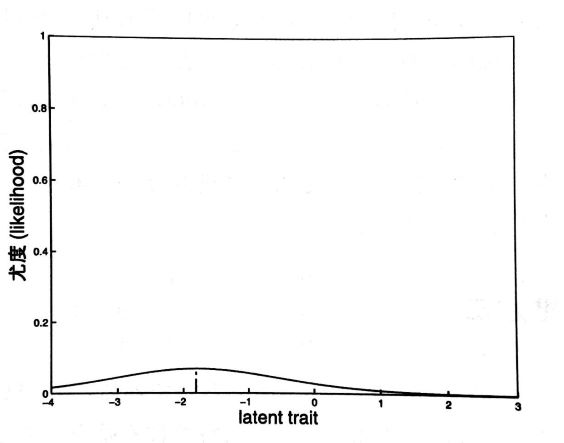
\includegraphics[bb = 50 250 1 1,scale = 0.45]{1.jpg}
\end{figure}
\begin{figure}[H]
  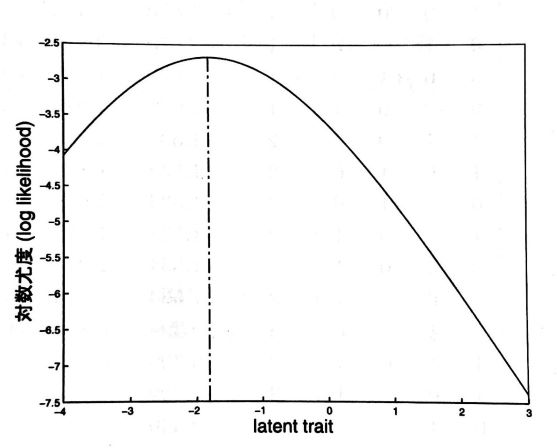
\includegraphics[bb = -500 150 1 1,scale = 0.45]{2.jpg}
\end{figure}
\begin{figure}[H]
  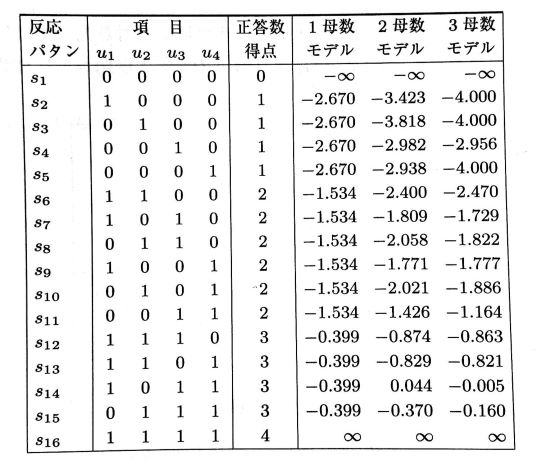
\includegraphics[bb = 50 520 1 1,scale = 0.5]{3.jpg}
\end{figure}
\begin{figure}[H]
  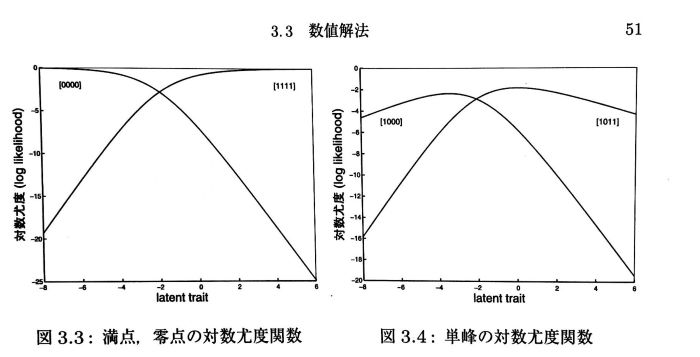
\includegraphics[bb = -150 820 1 1,scale = 0.5]{4.jpg}
\end{figure}
\newpage
\begin{figure}[H]
  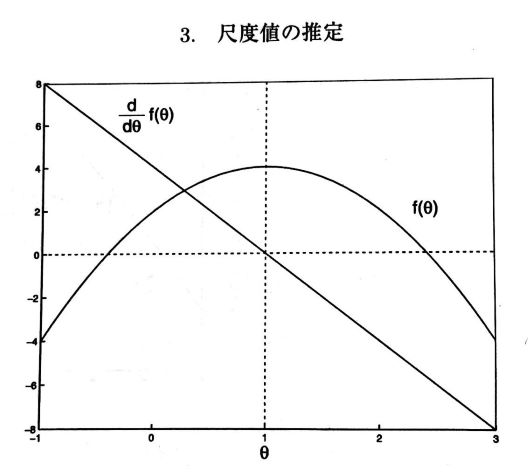
\includegraphics[bb = 50 500 1 1,scale = 0.45]{5.jpg}
\end{figure}
\begin{figure}[H]
  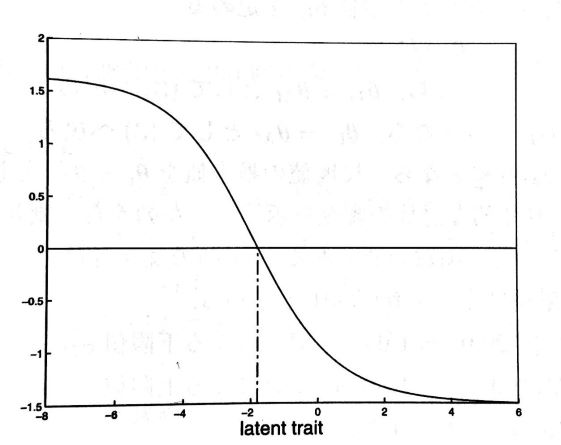
\includegraphics[bb = -500 400 1 1,scale = 0.45]{6.jpg}
\end{figure}






\end{document}
